\documentclass[grid,avery5388]{flashcards}
\usepackage{amssymb}
\usepackage[utf8]{inputenc}
\usepackage[T1]{fontenc}
\usepackage{verse}
\usepackage[version=3]{mhchem}
\usepackage{graphicx}
\settowidth{\versewidth}{It lies behind stars and under hills,}
\addtolength{\versewidth}{2em}
\usepackage{pgfplots}
\geometry{headheight=12pt}
\usepackage{fancyhdr}
\pagestyle{fancy}
\fancyhf{}
\renewcommand{\headrulewidth}{0pt}


\title{Conversion flashcards}
\author{Sam Robbins}

\cardbackstyle[\large]{plain}
\cardfrontstyle[\large]{headings}
%\cardbackstyle[\large]{headings}

\begin{document}

\begin{flashcard}[]{What are the three fundamental phases of integrated circuit design?
You should briefly explain what each phase does. [3]}

A \textbf{functional specification} $[\frac{1}{2}]$ of the chip is derived (this describes
exactly what the IC is supposed to do involving factors like chip area,
power, speed and cost $[\frac{1}{2}]$); the \textbf{register transfer level (RTL)} $[\frac{1}{2}]$ design
is then undertaken (the functional specification is used to describe
the exact behaviour of the digital circuits on the chip, as well as the
interconnections to inputs and outputs, with this description being in
terms of logic gates and interconnecting wires $[\frac{1}{2}]$); and then the RTL
design is \textbf{mapped to a physical layout} $[\frac{1}{2}]$ in silicon (specific physical
attributes must be respected; for example, it is crucial that appropriate
spacing between transistors is maintained in the physical layout $[\frac{1}{2}]$).
\end{flashcard}

\begin{flashcard}[]{What is a NAND-gate? Show how a NOT-gate, an AND-gate and an
OR-gate can be constructed using just NAND-gates. [10]}
A NAND-gate takes two inputs and outputs 0 if, and only if, both
inputs are 1 [1]. [2] for NOT-gate; [3] for AND-gate; [4] for OR-gate\\
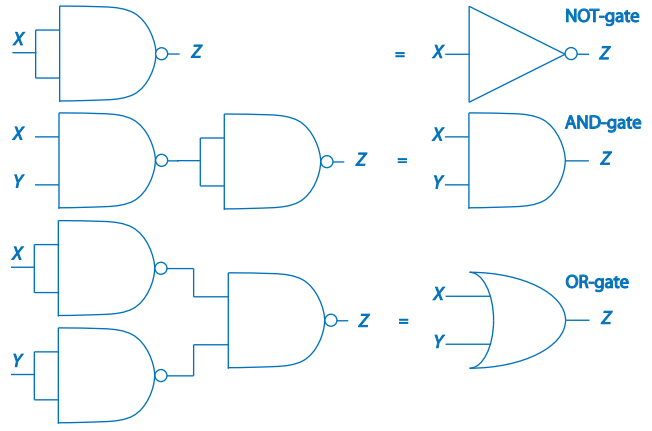
\includegraphics[width=8cm]{NAND.png}
\end{flashcard}

\begin{flashcard}[]{Build a circuit using NOT-, AND- and OR-gates that computes the
function with 3 Boolean inputs and where the output is 1 if, and only
if, there are an even number of 1’s in the input. [6]}
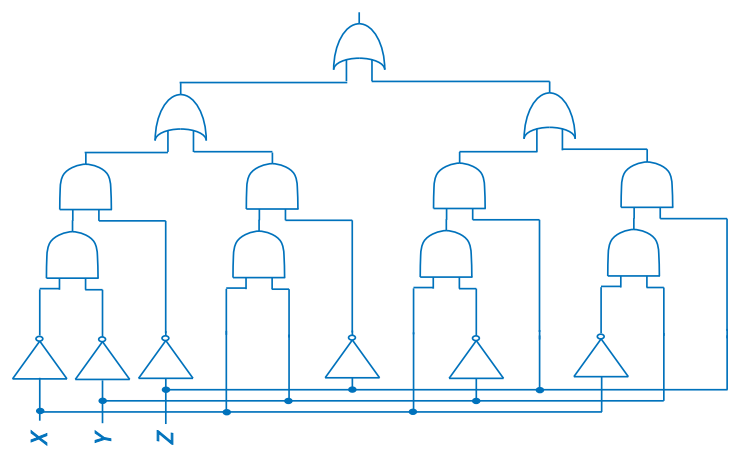
\includegraphics[width=11cm]{even.png}
\end{flashcard}


\begin{flashcard}[]{
What are a half-adder and a full-adder? Show how a full-adder can be
built using 2 half-adders. [7]
}
A half-adder takes x and y as inputs and computes the Boolean sum
of x and y, where the Boolean sum of a collection of inputs is 1 if, and
only if, an odd number of the inputs are 1, and also the resulting carry
bit, which is 1 if, and only if, both x and y are 1 [2]. A full-adder takes
x, y, and z as inputs and computes the Boolean sum of x, y, and z,
resulting in the sum-bit and the carry-bit [2].\\
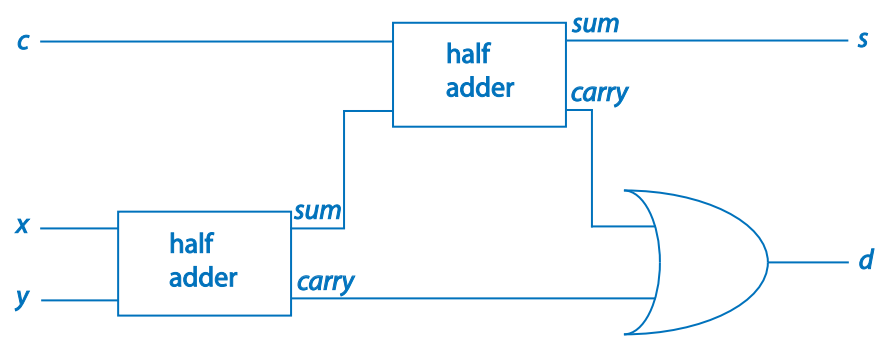
\includegraphics[width=8cm]{full_adder.png}
\end{flashcard}

\begin{flashcard}[]{Name three key components in a CPU microarchitecture and briefly
describe the purpose of each. [3]}

The \textbf{datapath} $[\frac{1}{2}]$ performs all the data processing operations and includes
the arithmetic logic unit (ALU), which is the part of the CPU
that performs all the arithmetic and logical operations on data, and a
limited number of memory locations called registers $[\frac{1}{2}]$. The \textbf{control}
$[\frac{1}{2}]$ tells the datapath, memory and input/output (I/O) devices what
to do (it is the conduit between the datapath and the main memory) $[\frac{1}{2}]$. A \textbf{cache} $[\frac{1}{2}]$ consists of small, fast and relatively expensive on-chip
memory and is used to store memory items that need to be regularly
accessed $[\frac{1}{2}]$.

\end{flashcard}


\begin{flashcard}[]{Name two types of bus within a CPU and explain the general purpose
of each. What is the width of a bus? Explain how the width of a bus
imposes memory or data limitations within a CPU. [6]}

Buses include a \textbf{data bus} $[\frac{1}{2}]$, an \textbf{address bus} $[\frac{1}{2}]$ and a \textbf{control bus} $[\frac{1}{2}]$. A data bus carries the contents of memory locations between the
processor and main memory $[\frac{1}{2}]$. The address bus holds addresses of
locations in main memory $[\frac{1}{2}]$. The control bus is used to transfer
information between the CPU and various other devices within the
processor $[\frac{1}{2}]$. The width of a bus is the number of parallel wires in
a bus [1]. The width of the data bus determines the word-size of the
computer [1]. The width of an address bus determines the size of
addressable memory [1].

\end{flashcard}

\begin{flashcard}[]{Explain carefully the four phases of the fetch-decode-fetch-execute processor cycle (be sure to explain the purpose of any CPU components
you happen to mention). [5]}


\end{flashcard}

\begin{flashcard}[]{Show different layers of abstraction in a modern computer system. [4]}
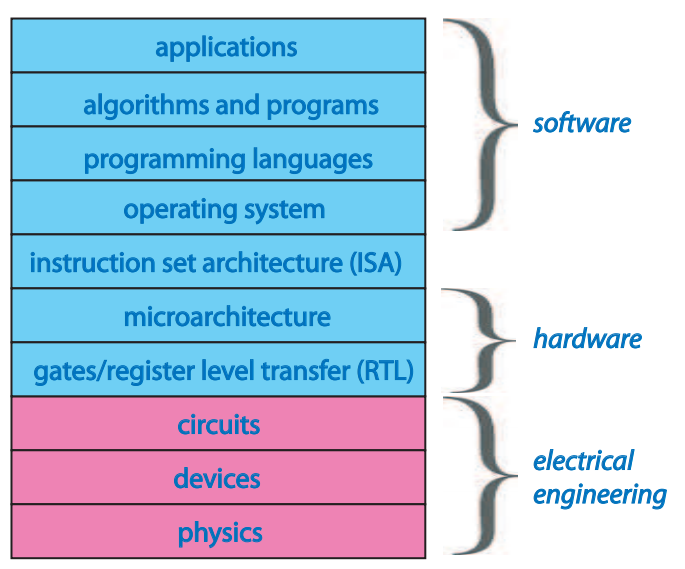
\includegraphics[width=8cm]{CSys.png}

\end{flashcard}



\end{document}